\PassOptionsToPackage{unicode=true}{hyperref} % options for packages loaded elsewhere
\PassOptionsToPackage{hyphens}{url}
%
\documentclass[australian,ignorenonframetext,aspectratio=169]{beamer}
\usepackage{pgfpages}
\setbeamertemplate{caption}[numbered]
\setbeamertemplate{caption label separator}{: }
\setbeamercolor{caption name}{fg=normal text.fg}
\beamertemplatenavigationsymbolsempty
% Prevent slide breaks in the middle of a paragraph:
\widowpenalties 1 10000
\raggedbottom
\setbeamertemplate{part page}{
\centering
\begin{beamercolorbox}[sep=16pt,center]{part title}
  \usebeamerfont{part title}\insertpart\par
\end{beamercolorbox}
}
\setbeamertemplate{section page}{
\centering
\begin{beamercolorbox}[sep=12pt,center]{part title}
  \usebeamerfont{section title}\insertsection\par
\end{beamercolorbox}
}
\setbeamertemplate{subsection page}{
\centering
\begin{beamercolorbox}[sep=8pt,center]{part title}
  \usebeamerfont{subsection title}\insertsubsection\par
\end{beamercolorbox}
}
\AtBeginPart{
  \frame{\partpage}
}
\AtBeginSection{
  \ifbibliography
  \else
    \frame{\sectionpage}
  \fi
}
\AtBeginSubsection{
  \frame{\subsectionpage}
}
\usepackage{lmodern}
\usepackage{amssymb,amsmath}
\usepackage{ifxetex,ifluatex}
\usepackage{fixltx2e} % provides \textsubscript
\ifnum 0\ifxetex 1\fi\ifluatex 1\fi=0 % if pdftex
  \usepackage[T1]{fontenc}
  \usepackage[utf8]{inputenc}
  \usepackage{textcomp} % provides euro and other symbols
\else % if luatex or xelatex
  \usepackage{unicode-math}
  \defaultfontfeatures{Ligatures=TeX,Scale=MatchLowercase}
\fi
\usetheme[]{metropolis}
% use upquote if available, for straight quotes in verbatim environments
\IfFileExists{upquote.sty}{\usepackage{upquote}}{}
% use microtype if available
\IfFileExists{microtype.sty}{%
\usepackage[]{microtype}
\UseMicrotypeSet[protrusion]{basicmath} % disable protrusion for tt fonts
}{}
\IfFileExists{parskip.sty}{%
\usepackage{parskip}
}{% else
\setlength{\parindent}{0pt}
\setlength{\parskip}{6pt plus 2pt minus 1pt}
}
\usepackage{hyperref}
\hypersetup{
            pdftitle={Multiple regression \& Gauss-Markov Theorem},
            pdfauthor={Luis Castro-de-Araujo},
            pdfborder={0 0 0},
            breaklinks=true}
\urlstyle{same}  % don't use monospace font for urls
\newif\ifbibliography
\usepackage{color}
\usepackage{fancyvrb}
\newcommand{\VerbBar}{|}
\newcommand{\VERB}{\Verb[commandchars=\\\{\}]}
\DefineVerbatimEnvironment{Highlighting}{Verbatim}{commandchars=\\\{\}}
% Add ',fontsize=\small' for more characters per line
\usepackage{framed}
\definecolor{shadecolor}{RGB}{248,248,248}
\newenvironment{Shaded}{\begin{snugshade}}{\end{snugshade}}
\newcommand{\AlertTok}[1]{\textcolor[rgb]{0.94,0.16,0.16}{#1}}
\newcommand{\AnnotationTok}[1]{\textcolor[rgb]{0.56,0.35,0.01}{\textbf{\textit{#1}}}}
\newcommand{\AttributeTok}[1]{\textcolor[rgb]{0.77,0.63,0.00}{#1}}
\newcommand{\BaseNTok}[1]{\textcolor[rgb]{0.00,0.00,0.81}{#1}}
\newcommand{\BuiltInTok}[1]{#1}
\newcommand{\CharTok}[1]{\textcolor[rgb]{0.31,0.60,0.02}{#1}}
\newcommand{\CommentTok}[1]{\textcolor[rgb]{0.56,0.35,0.01}{\textit{#1}}}
\newcommand{\CommentVarTok}[1]{\textcolor[rgb]{0.56,0.35,0.01}{\textbf{\textit{#1}}}}
\newcommand{\ConstantTok}[1]{\textcolor[rgb]{0.00,0.00,0.00}{#1}}
\newcommand{\ControlFlowTok}[1]{\textcolor[rgb]{0.13,0.29,0.53}{\textbf{#1}}}
\newcommand{\DataTypeTok}[1]{\textcolor[rgb]{0.13,0.29,0.53}{#1}}
\newcommand{\DecValTok}[1]{\textcolor[rgb]{0.00,0.00,0.81}{#1}}
\newcommand{\DocumentationTok}[1]{\textcolor[rgb]{0.56,0.35,0.01}{\textbf{\textit{#1}}}}
\newcommand{\ErrorTok}[1]{\textcolor[rgb]{0.64,0.00,0.00}{\textbf{#1}}}
\newcommand{\ExtensionTok}[1]{#1}
\newcommand{\FloatTok}[1]{\textcolor[rgb]{0.00,0.00,0.81}{#1}}
\newcommand{\FunctionTok}[1]{\textcolor[rgb]{0.00,0.00,0.00}{#1}}
\newcommand{\ImportTok}[1]{#1}
\newcommand{\InformationTok}[1]{\textcolor[rgb]{0.56,0.35,0.01}{\textbf{\textit{#1}}}}
\newcommand{\KeywordTok}[1]{\textcolor[rgb]{0.13,0.29,0.53}{\textbf{#1}}}
\newcommand{\NormalTok}[1]{#1}
\newcommand{\OperatorTok}[1]{\textcolor[rgb]{0.81,0.36,0.00}{\textbf{#1}}}
\newcommand{\OtherTok}[1]{\textcolor[rgb]{0.56,0.35,0.01}{#1}}
\newcommand{\PreprocessorTok}[1]{\textcolor[rgb]{0.56,0.35,0.01}{\textit{#1}}}
\newcommand{\RegionMarkerTok}[1]{#1}
\newcommand{\SpecialCharTok}[1]{\textcolor[rgb]{0.00,0.00,0.00}{#1}}
\newcommand{\SpecialStringTok}[1]{\textcolor[rgb]{0.31,0.60,0.02}{#1}}
\newcommand{\StringTok}[1]{\textcolor[rgb]{0.31,0.60,0.02}{#1}}
\newcommand{\VariableTok}[1]{\textcolor[rgb]{0.00,0.00,0.00}{#1}}
\newcommand{\VerbatimStringTok}[1]{\textcolor[rgb]{0.31,0.60,0.02}{#1}}
\newcommand{\WarningTok}[1]{\textcolor[rgb]{0.56,0.35,0.01}{\textbf{\textit{#1}}}}
\usepackage{longtable,booktabs}
\usepackage{caption}
% These lines are needed to make table captions work with longtable:
\makeatletter
\def\fnum@table{\tablename~\thetable}
\makeatother
\usepackage{graphicx,grffile}
\makeatletter
\def\maxwidth{\ifdim\Gin@nat@width>\linewidth\linewidth\else\Gin@nat@width\fi}
\def\maxheight{\ifdim\Gin@nat@height>\textheight\textheight\else\Gin@nat@height\fi}
\makeatother
% Scale images if necessary, so that they will not overflow the page
% margins by default, and it is still possible to overwrite the defaults
% using explicit options in \includegraphics[width, height, ...]{}
\setkeys{Gin}{width=\maxwidth,height=\maxheight,keepaspectratio}
\setlength{\emergencystretch}{3em}  % prevent overfull lines
\providecommand{\tightlist}{%
  \setlength{\itemsep}{0pt}\setlength{\parskip}{0pt}}
\setcounter{secnumdepth}{0}

% set default figure placement to htbp
\makeatletter
\def\fps@figure{htbp}
\makeatother

\usepackage{navigator}
\embeddedfile{project}{2022-presentation.Rmd}
 \usepackage{appendixnumberbeamer}
 \usepackage{roboto}
\usepackage[font={footnotesize}]{caption}
\setbeamerfont{footnote}{size=\tiny}
\metroset{sectionpage=progressbar, titleformat=smallcaps}
\setbeamercolor{itemize item}{fg=vcuyellow}
\setbeamercolor{itemize subitem}{fg=vcuyellow}
\setbeamercolor{itemize subsubitem}{fg=vcuyellow}
 \setbeamertemplate{itemize item}[circle]
 \setbeamertemplate{itemize subitem}[square]
 \setbeamertemplate{itemize subsubitem}[triangle]
 \titlegraphic{%
 \hfill
\includegraphics[width=3cm,height=1.6cm,keepaspectratio]{style/VCU-Logo.png}}
 \definecolor{vcuyellow}{HTML}{FDBD10}
\setbeamercolor{palette primary}{fg=vcuyellow, bg=black}
 \setbeamercolor{frametitle}{fg=vcuyellow, bg=black}
 \setbeamercolor{titlelike}{fg=black}
 \setbeamercolor{titlepage}{fg=black, bg=vcuyellow}
 \setbeamercolor{footnote}{bg=black}
 \setbeamercolor{normal text}{fg=black}
 \setbeamercolor{block title}{fg=black, bg=vcuyellow!40!white}
 \setbeamercolor{alerted text}{fg=red}
 \setbeamercolor{example text}{fg=black}
 \setbeamercolor{title separator}{fg = vcuyellow, bg=vcuyellow}
\setbeamercolor{progress bar}{bg=white, fg=vcuyellow}
\setbeamercolor{progress bar in head/foot}{bg=white, fg=vcuyellow}
 \setbeamercolor{progress bar in section page}{bg=white, fg=vcuyellow}
\makeatletter
\newsavebox{\mybox}
\setbeamertemplate{frametitle}{%
 \nointerlineskip%
 \savebox{\mybox}{%
     \begin{beamercolorbox}[%
         wd=\paperwidth,%
         sep=0pt,%
         leftskip=\metropolis@frametitle@padding,%
         rightskip=\metropolis@frametitle@padding,%
       ]{frametitle}%
     \metropolis@frametitlestrut@start\insertframetitle\metropolis@frametitlestrut@end%
     \end{beamercolorbox}%
   }
 \begin{beamercolorbox}[%
     wd=\paperwidth,%
     sep=0pt,%
     leftskip=\metropolis@frametitle@padding,%
     rightskip=\metropolis@frametitle@padding,%
   ]{frametitle}%
 \metropolis@frametitlestrut@start\insertframetitle\metropolis@frametitlestrut@end%
 \hfill%
 \raisebox{-\metropolis@frametitle@padding}{
\includegraphics[height=\dimexpr\ht\mybox+\metropolis@frametitle@padding\relax]{style/VCU-Logo.png}}%
   \hspace*{-\metropolis@frametitle@padding}
 \end{beamercolorbox}%
}
\makeatother
 \makeatletter
 \pretocmd{\beamer@reseteecodes}{%
   \ifbool{metropolis@standout}{
     \endgroup
     \boolfalse{metropolis@standout}
   }{}
 }{}{}
 \makeatother
\ifnum 0\ifxetex 1\fi\ifluatex 1\fi=0 % if pdftex
  \usepackage[shorthands=off,main=australian]{babel}
\else
  % load polyglossia as late as possible as it *could* call bidi if RTL lang (e.g. Hebrew or Arabic)
  \usepackage{polyglossia}
  \setmainlanguage[variant=australian]{english}
\fi

\title{Multiple regression \& Gauss-Markov Theorem}
\author{Luis Castro-de-Araujo\footnote<.->{Post-doc T32.
  \href{mailto:luis.araujo@vcuhealth.org}{\nolinkurl{luis.araujo@vcuhealth.org}}\\}}
\providecommand{\institute}[1]{}
\institute{Virginia Institute for Psychiatric and Behavioral Genetics}
\date{11/07/2022}

\begin{document}
\frame{\titlepage}

\begin{frame}
\tableofcontents[hideallsubsections]
\end{frame}
\begin{frame}

\section{Linear regression recap}

\end{frame}

\begin{frame}{Regression}
\protect\hypertarget{regression}{}

\begin{itemize}
\tightlist
\item
  Technique used for the modeling and analysis of numerical
  data\footnote<.->{Akey, 2020, ``Regression,'' (Washington 2020).}
\item
  Exploits the relationship between two or more variables so that we can
  gain information about one of them through knowing values of the other
\item
  Regression can be used for prediction, estimation, hypothesis testing,
  and modeling causal relationships
\end{itemize}

\end{frame}

\begin{frame}[standout]{}
\protect\hypertarget{section}{}

\begin{itemize}
\tightlist
\item
  It is all about describing relationships between variables
\end{itemize}

\end{frame}

\begin{frame}{The culprit}
\protect\hypertarget{the-culprit}{}

\begin{columns}[T]
\begin{column}{0.5\textwidth}
\begin{block}{Bio}

\begin{itemize}
\tightlist
\item
  30 April 1777 - 23 April 1855
\item
  Worked in the theorem around 1794
\item
  17 years old!\footnote<.->{``Carl Friedrich Gauss,'' (2022),
    \emph{Wikipedia}.}
\end{itemize}

\end{block}
\end{column}

\begin{column}{0.5\textwidth}
\begin{block}{Carl Friedrich Gauss}

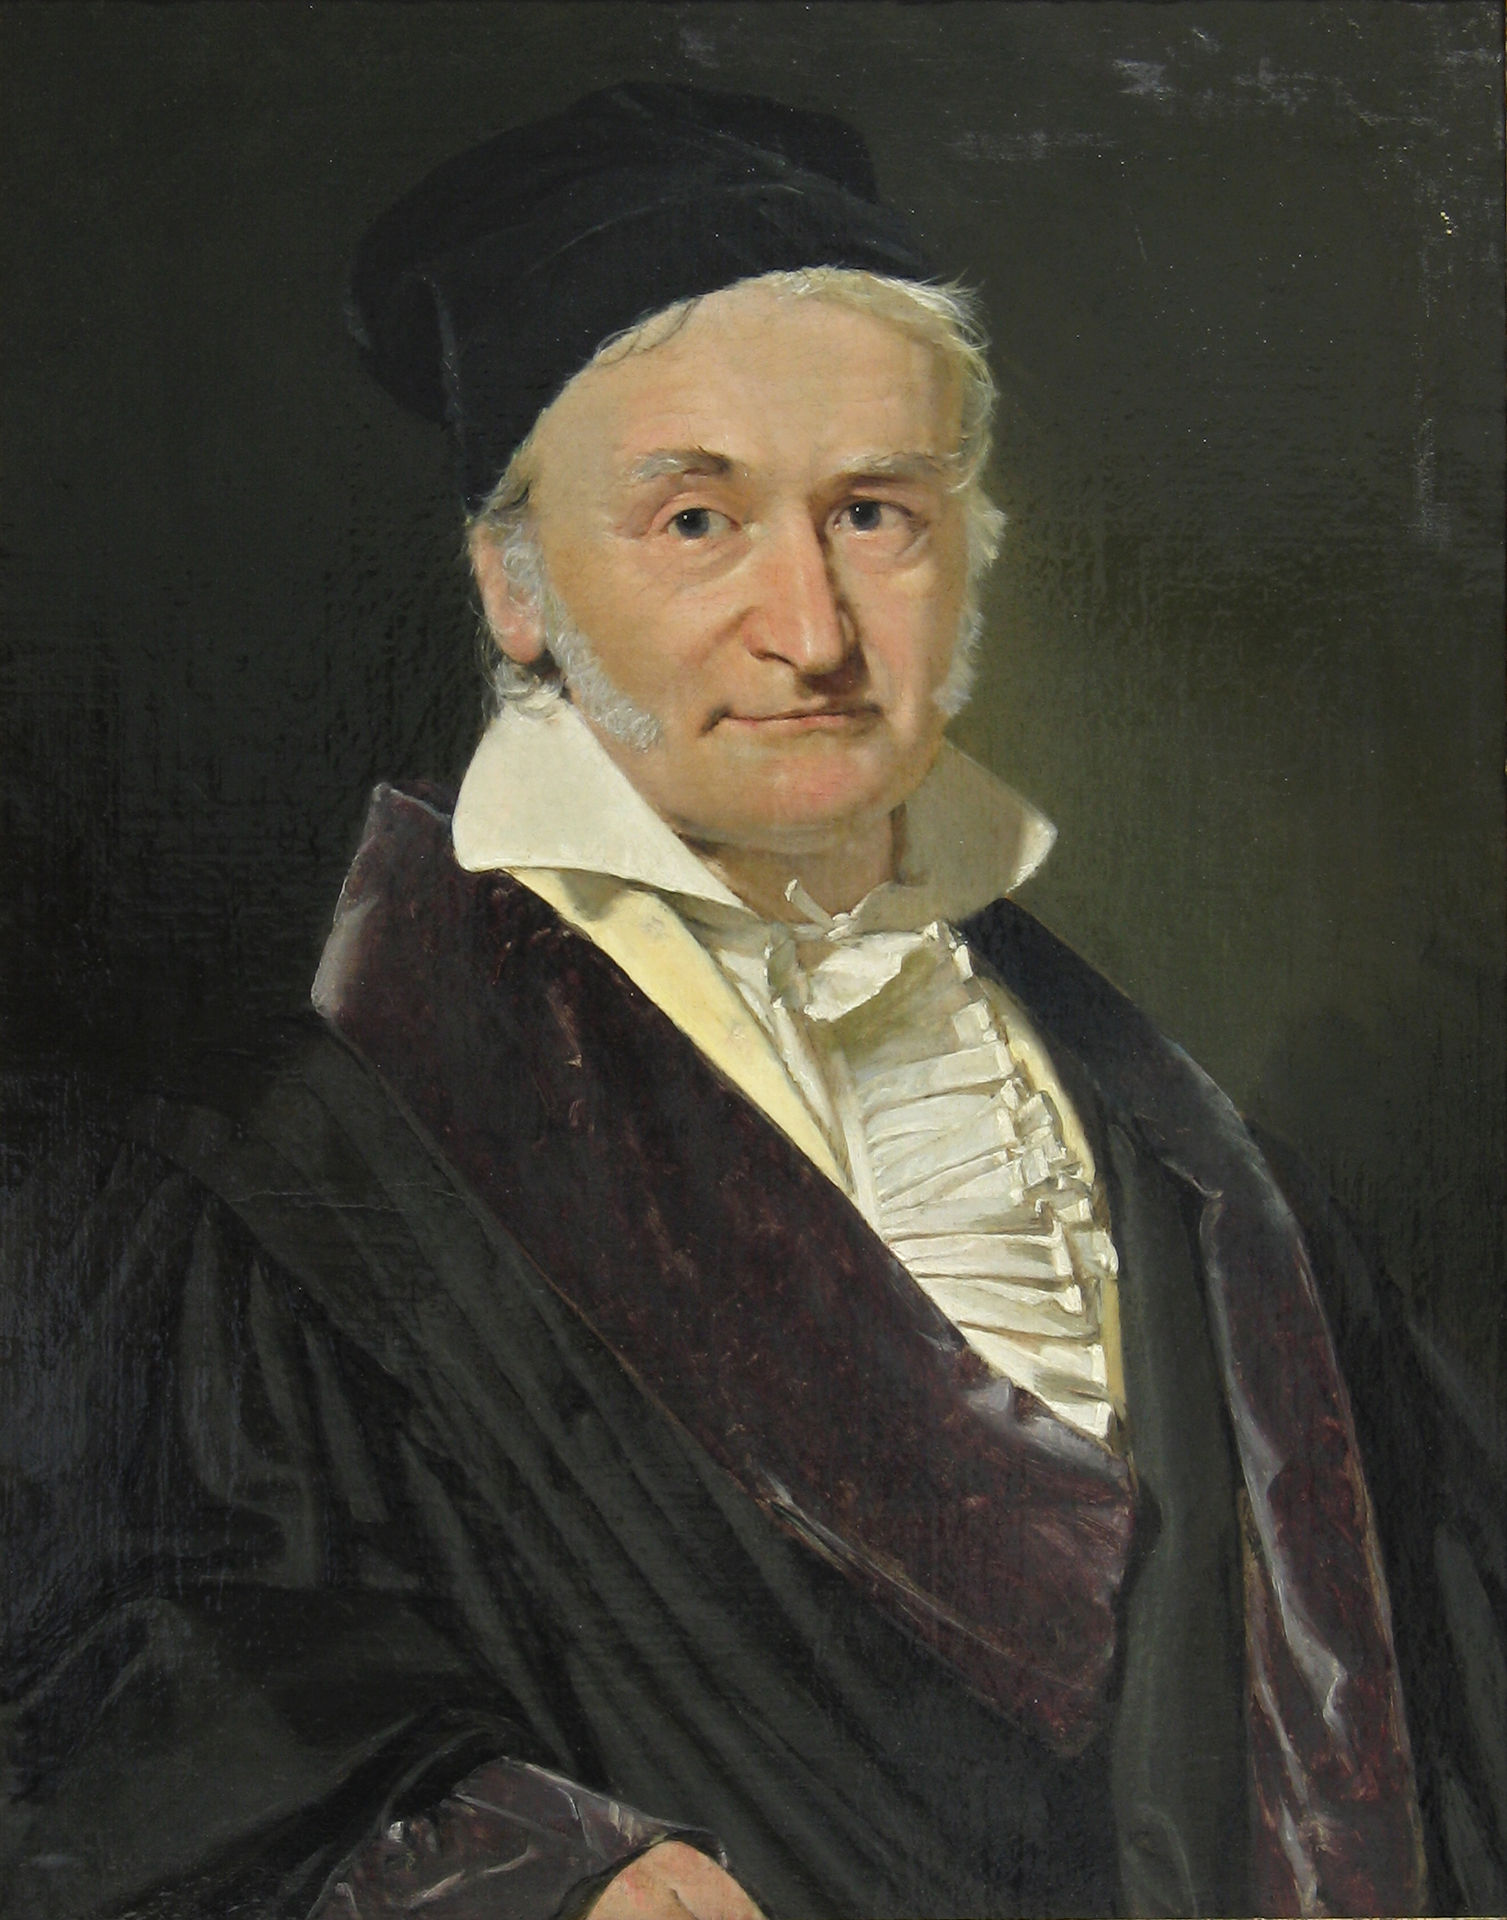
\includegraphics[width=1\linewidth]{../graphs/gauss}

\end{block}
\end{column}
\end{columns}

\end{frame}

\begin{frame}[fragile]{Before him, description of relationship was not
systematic}
\protect\hypertarget{before-him-description-of-relationship-was-not-systematic}{}

\begin{columns}[T]
\begin{column}{0.5\textwidth}
\small

\begin{Shaded}
\begin{Highlighting}[]
\KeywordTok{set.seed}\NormalTok{(}\DecValTok{42}\NormalTok{)}
\NormalTok{x \textless{}{-}}\StringTok{ }\KeywordTok{rnorm}\NormalTok{(}\DecValTok{100}\NormalTok{)}
\NormalTok{y \textless{}{-}}\StringTok{ }\DecValTok{2} \OperatorTok{*}\StringTok{ }\NormalTok{x }\OperatorTok{+}\StringTok{ }\KeywordTok{rnorm}\NormalTok{(}\DecValTok{100}\NormalTok{, }\DataTypeTok{sd =} \FloatTok{0.8}\NormalTok{)}
\KeywordTok{plot}\NormalTok{(x, y, }\DataTypeTok{xlab =} \StringTok{"x"}\NormalTok{, }\DataTypeTok{ylab =} \StringTok{"y"}\NormalTok{)}
\end{Highlighting}
\end{Shaded}
\end{column}

\begin{column}{0.5\textwidth}
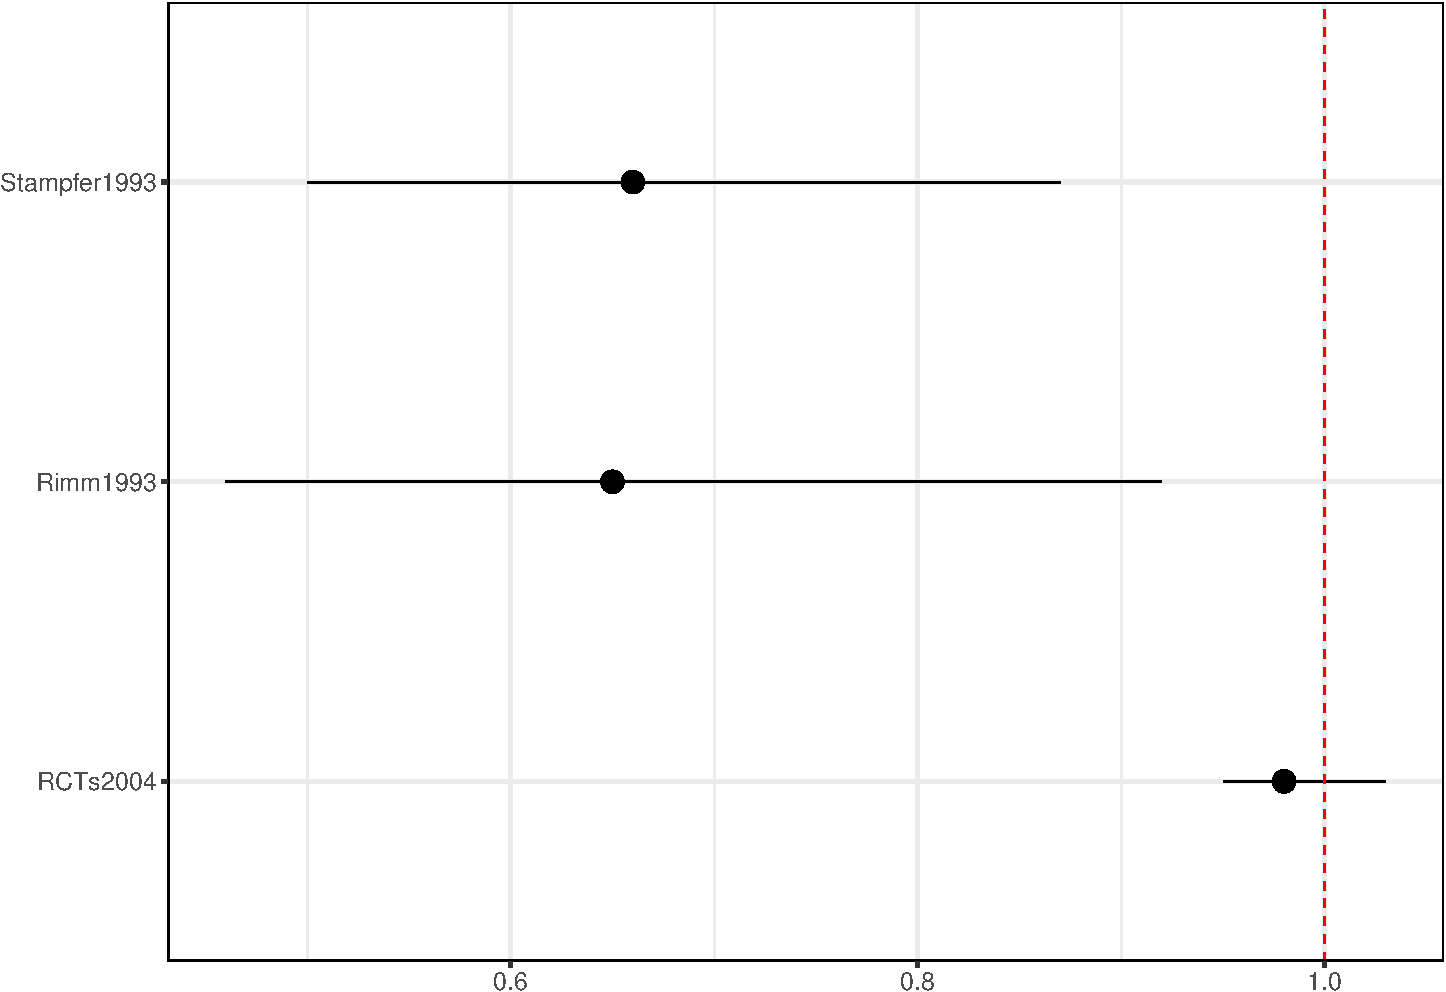
\includegraphics{../graphs/unnamed-chunk-3-1.pdf}
\end{column}
\end{columns}

\end{frame}

\begin{frame}{Regression Lingo\footnote<.->{Joshua Akey, ``Regression.''}}
\protect\hypertarget{regression-lingo-akeyregression2020}{}

\[Y = X1 + X2 + X3\]

\begin{longtable}[]{@{}ll@{}}
\toprule
Left of expression & Right of expression\tabularnewline
\midrule
\endhead
Dependent Variable & Independent Variable\tabularnewline
Outcome Variable & Predictor Variable\tabularnewline
Response Variable & Explanatory Variable\tabularnewline
\bottomrule
\end{longtable}

\end{frame}

\begin{frame}{Why Linear Regression?}
\protect\hypertarget{why-linear-regression}{}

\begin{itemize}
\tightlist
\item
  Suppose we want to model the dependent variable Y in terms of three
  predictors, X1, X2, X3\footnote<.->{Ibid.}
\end{itemize}

\[Y = f(X1, X2, X3)\]

\begin{itemize}
\tightlist
\item
  We usually have to assume that it has some restricted form, such as
  linear + error
\end{itemize}

\[Y = X1 + X2 + X3 + \epsilon\]

\end{frame}

\begin{frame}{Linear Regression is a Probabilistic Model}
\protect\hypertarget{linear-regression-is-a-probabilistic-model}{}

\begin{columns}[T]
\begin{column}{0.5\textwidth}
\begin{itemize}
\tightlist
\item
  Much of mathematics is devoted to studying variables that are
  deterministically related to one another\footnote<.->{Ibid.}
\end{itemize}

\[y = \beta_0 + \beta_1x\]

\begin{itemize}
\tightlist
\item
  But we're interested in understanding the relationship between
  variables related in a nondeterministic fashion.
\end{itemize}
\end{column}

\begin{column}{0.5\textwidth}
\begin{center}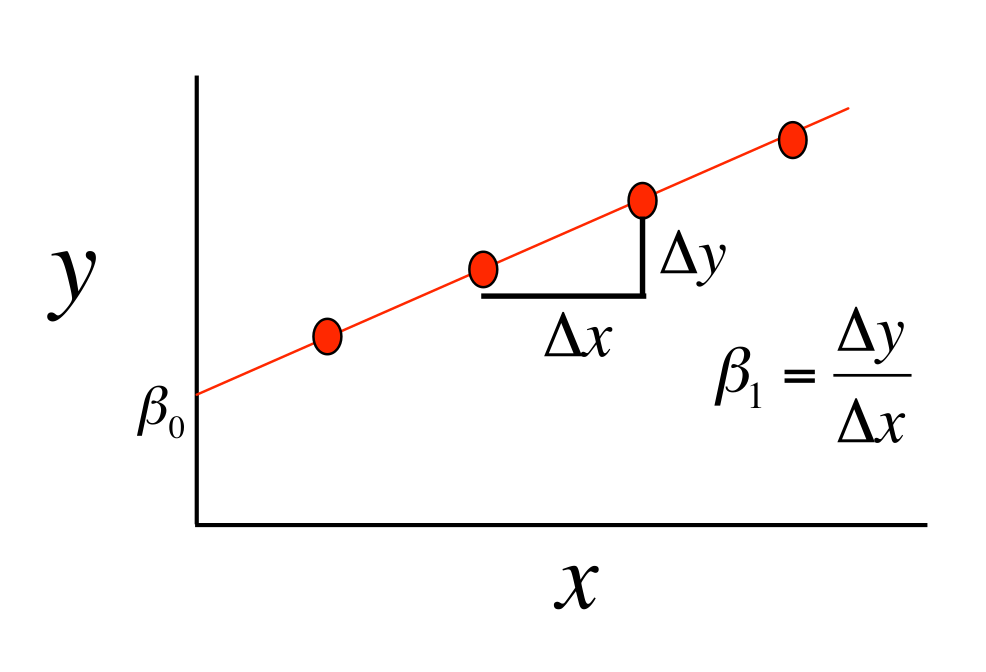
\includegraphics[width=1\linewidth]{../graphs/ari} \end{center}
\end{column}
\end{columns}

\end{frame}

\begin{frame}{A Linear Probabilistic Model}
\protect\hypertarget{a-linear-probabilistic-model}{}

\begin{columns}[T]
\begin{column}{0.5\textwidth}
\tiny

\begin{itemize}
\tightlist
\item
  There exists parameters \(\beta_0\), \(\beta_1\), and \(\sigma^2\) ,
  such that for any fixed value of the independent variable x, the
  dependent variable is related to x through the model
  equation\footnote<.->{Ibid.}
\end{itemize}

\[y = \beta_0 + \beta_1x + \epsilon\]

\begin{itemize}
\tightlist
\item
  The error term \(\epsilon\) is a random variable with mean 0 and
  constant variance \(\sigma^2\)
\end{itemize}
\end{column}

\begin{column}{0.5\textwidth}
Or, more succinctly,

\[\left[\begin{array}{c}
y_1 \\
y_2 \\
\vdots \\
y_n
\end{array}\right]=\left[\begin{array}{cc}
1 & x_1 \\
1 & x_2 \\
\vdots & \vdots \\
1 & x_n
\end{array}\right]\left[\begin{array}{c}
\beta_0 \\
\beta_1
\end{array}\right]+\left[\begin{array}{c}
\varepsilon_1 \\
\varepsilon_2 \\
\vdots \\
\varepsilon_n
\end{array}\right]\]
\end{column}
\end{columns}

\end{frame}

\begin{frame}{A substantive example}
\protect\hypertarget{a-substantive-example}{}

\begin{block}{From a bad model\footnote<.->{Wilber, ``Linear
  Regression,'' \emph{MLU-Explain}.}}

\begin{center}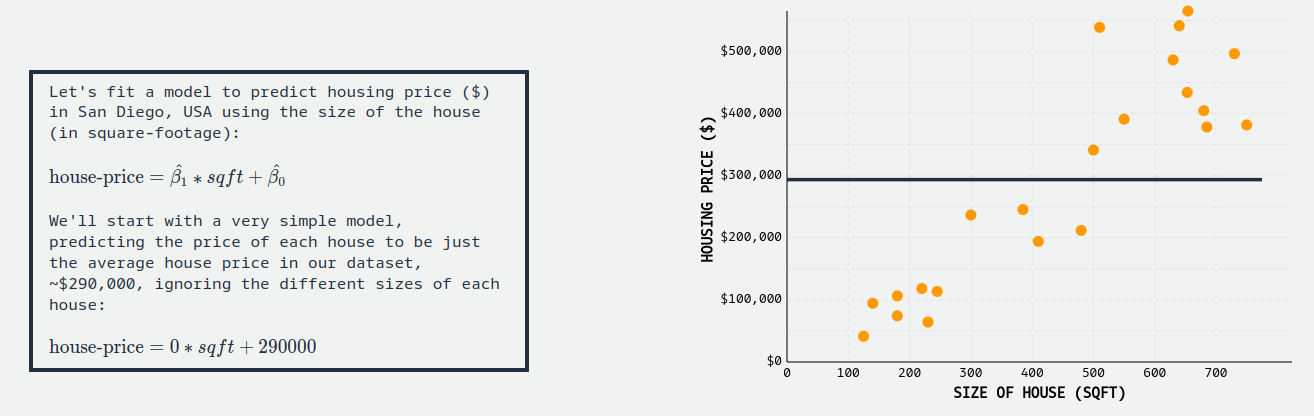
\includegraphics[width=1\linewidth]{../graphs/predict-1} \end{center}

\end{block}

\end{frame}

\begin{frame}{In other words}
\protect\hypertarget{in-other-words}{}

\begin{center}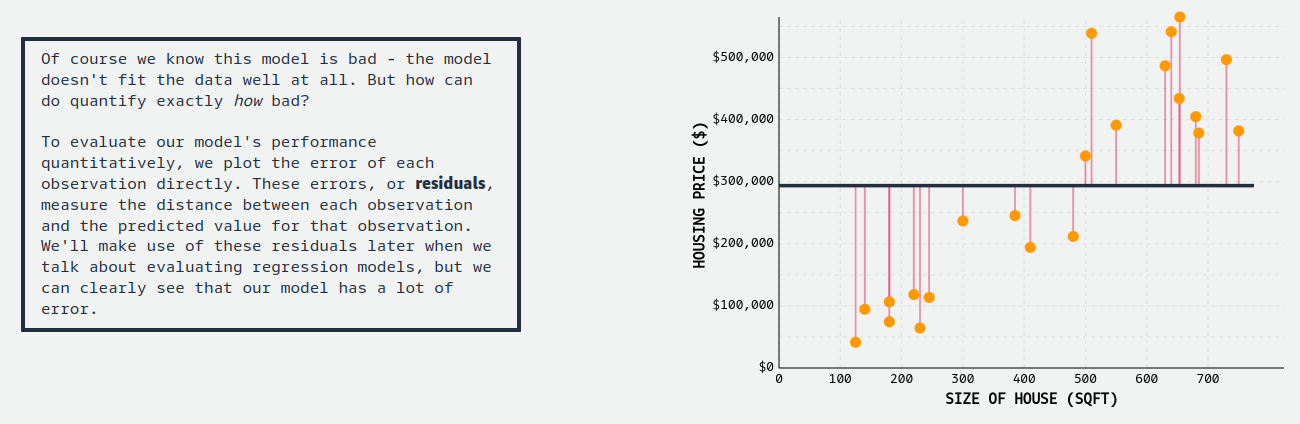
\includegraphics[width=1\linewidth]{../graphs/predict-2} \end{center}

\end{frame}

\begin{frame}{In other words}
\protect\hypertarget{in-other-words-1}{}

\begin{center}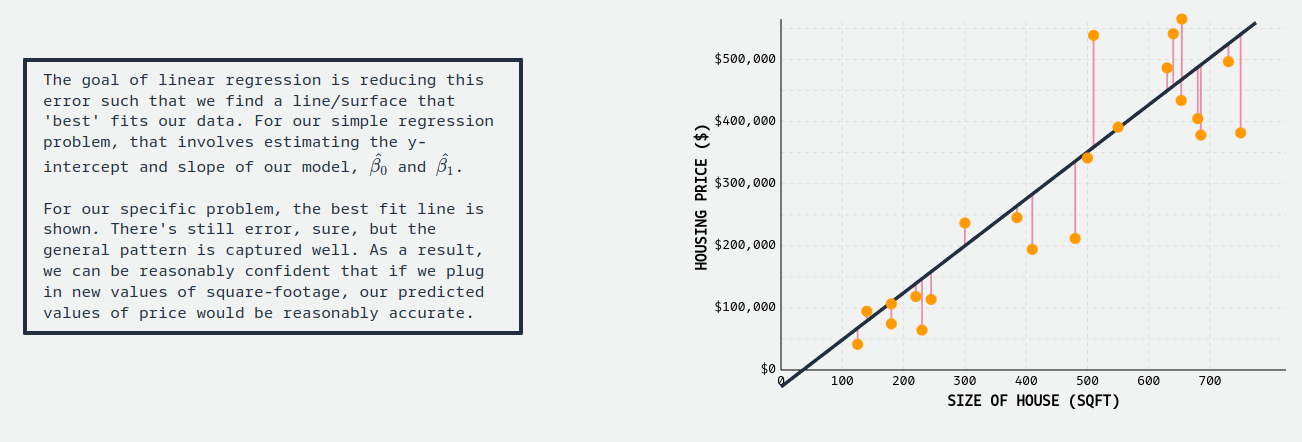
\includegraphics[width=1\linewidth]{../graphs/predict-3} \end{center}

\end{frame}

\begin{frame}{In other words}
\protect\hypertarget{in-other-words-2}{}

\begin{block}{To the best \textbf{possible} model\footnote<.->{Ibid.}}

\begin{center}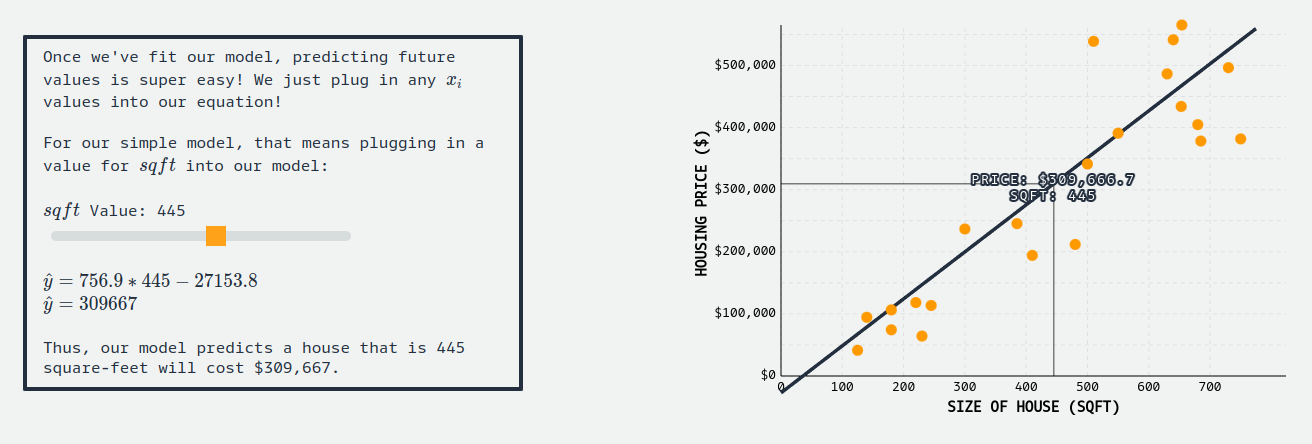
\includegraphics[width=1\linewidth]{../graphs/prediction-4} \end{center}

\end{block}

\end{frame}

\begin{frame}{Implications}
\protect\hypertarget{implications}{}

\begin{itemize}
\item
  The \textbf{expected} value of Y is a linear function of X, but for
  fixed x, the variable Y differs from its expected value by a random
  amount\footnote<.->{Ibid.}
\item
  Formally, let x* denote a particular value of the independent variable
  x, then our linear probabilistic model says:
\end{itemize}

\[E(Y|x^*) = \mu_{Y|x^*}\text{ = mean value of Y when x is x*}\]

\[V(Y|x^*) = \sigma^2_{Y|x^*}\text{= variance of Y when x is x*}\] ~

\end{frame}

\begin{frame}{Graphical Interpretation}
\protect\hypertarget{graphical-interpretation}{}

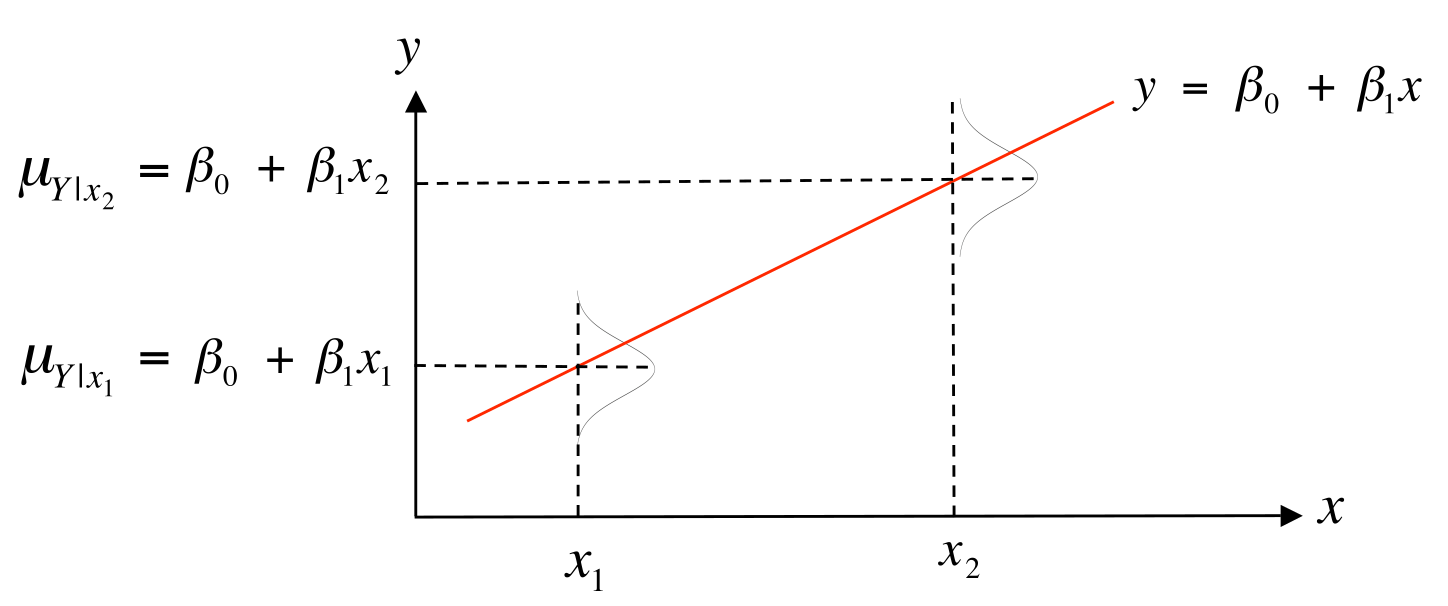
\includegraphics[width=4.83in]{../graphs/regression}

\begin{itemize}
\tightlist
\item
  For example, if x = height and y = weight then \(\mu_{Y|x^*}=60\) is
  the average weight for all individuals 60 inches tall in the
  population
\end{itemize}

\end{frame}

\begin{frame}{Estimating Model Parameters}
\protect\hypertarget{estimating-model-parameters}{}

\begin{columns}[T]
\begin{column}{0.5\textwidth}
\begin{itemize}
\tightlist
\item
  Point estimates of \(\hat{\beta_0}\) and \(\hat{\beta_1}\) are
  obtained by the principle of least squares
\end{itemize}

\[f(\beta_0, \beta_1) = \sum_{i=1}^n (y_i - \beta_0 - \beta_1x_i)^2\]
\end{column}

\begin{column}{0.5\textwidth}
\begin{center}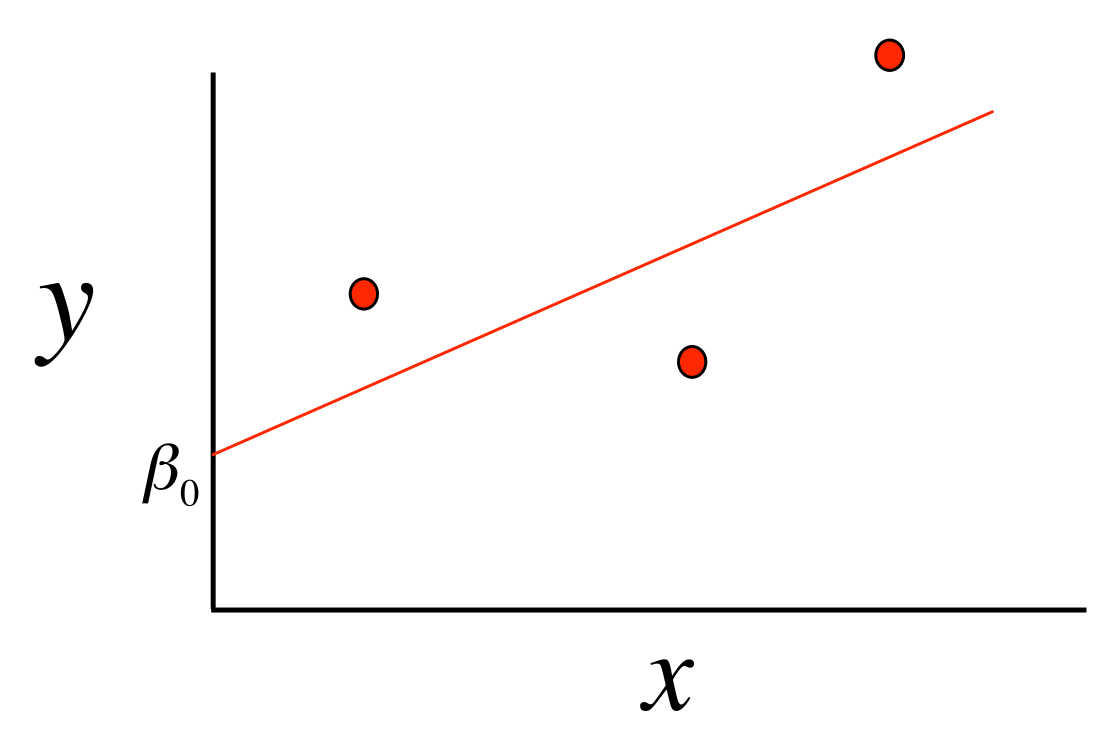
\includegraphics[width=1\linewidth]{../graphs/estimating} \end{center}
\end{column}
\end{columns}

\end{frame}

\begin{frame}{Predicted and Residual Values}
\protect\hypertarget{predicted-and-residual-values}{}

\begin{columns}[T]
\begin{column}{0.5\textwidth}
\tiny

\begin{itemize}
\tightlist
\item
  \textbf{Predicted} or fitted, values of y predicted by the
  least-squares regression line obtained by plugging in
  x1,x2,\ldots{},xn into the estimated regression line
\end{itemize}

\[\hat{y_1} = \hat{\beta_0} + \hat{\beta_1}x_1\]
\[\hat{y_2} = \hat{\beta_0} + \hat{\beta_1}x_2\]

\begin{itemize}
\tightlist
\item
  \textbf{Residuals} are the deviations of observed and predicted values
\end{itemize}

\[e_1 = y_1 - \hat{y_1}\] \[e_2 = y_2 - \hat{y_2}\]
\end{column}

\begin{column}{0.5\textwidth}
\begin{center}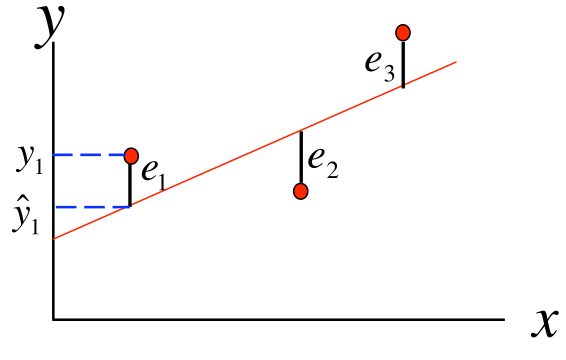
\includegraphics[width=1\linewidth]{../graphs/predicted} \end{center}
\end{column}
\end{columns}

\end{frame}

\begin{frame}{Residuals Are Useful!}
\protect\hypertarget{residuals-are-useful}{}

\begin{itemize}
\tightlist
\item
  They allow us to calculate the error sum of squares (SSE):
\end{itemize}

\[SSE = \sum_{i=1}^n (e_i)^2 = \sum_{i=1}^n (y_i - \hat{y_i})^2\]

\begin{itemize}
\tightlist
\item
  Which in turn allows us to estimate \(\sigma^2\):
\end{itemize}

\[\hat{\sigma^2} = \frac{SSE}{n-2}\]

\begin{itemize}
\tightlist
\item
  As well as the \textbf{coefficient of determination}:
\end{itemize}

\[R^2 = 1 - \frac{SSE}{SST};  SST = \sum_{i=1}^n (y_i - \bar{y})^2\]

\end{frame}

\begin{frame}{Binary variable}
\protect\hypertarget{binary-variable}{}

\begin{columns}[T]
\begin{column}{0.5\textwidth}
\begin{center}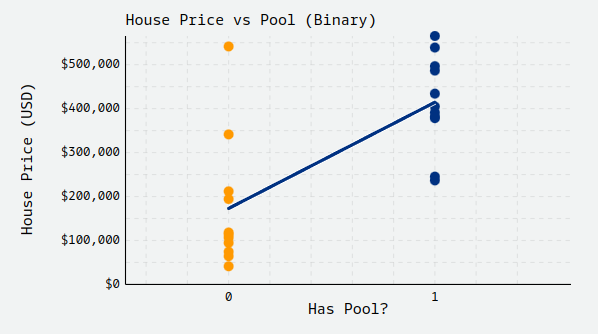
\includegraphics[width=1\linewidth]{../graphs/interpret-1} \end{center}

\(\begin{aligned} \text{house price} = 172893 + 241582 * pool \end{aligned}\)

\begin{itemize}
\tightlist
\item
  summarizes the difference in average housing prices between houses
  with and without pools
\end{itemize}
\end{column}

\begin{column}{0.5\textwidth}
\small

\begin{itemize}
\item
  The intercept, \$172,893, is the average predicted price for houses
  that do not have swimming pools.
\item
  To find the average price predicted price for houses with pools, we
  simply plug in pool=1 to obtain \$172,893 + \$241,582 * 1 = \$414,475.
\item
  The difference between these two subpopulation means is equal to the
  coefficient on pool. Houses with pools cost \$241,582 more on average
  than houses that do not have pools.
\end{itemize}
\end{column}
\end{columns}

\end{frame}

\begin{frame}{One continuous variable}
\protect\hypertarget{one-continuous-variable}{}

\begin{columns}[T]
\begin{column}{0.5\textwidth}
\begin{center}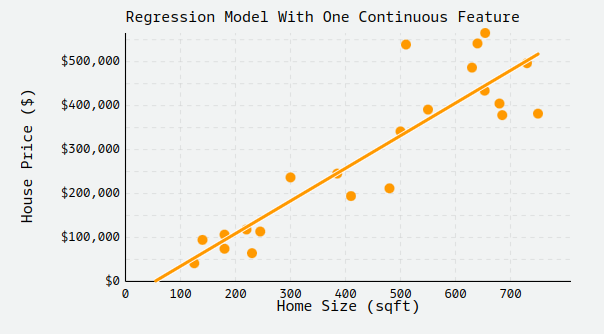
\includegraphics[width=1\linewidth]{../graphs/interpret-2} \end{center}

house price=-39591+742*sqft

\begin{itemize}
\tightlist
\item
  summarizes the average house prices across differently sized houses as
  measured in square feet.
\end{itemize}
\end{column}

\begin{column}{0.5\textwidth}
\small

\begin{itemize}
\item
  The coefficient, \$742, represents the average difference in housing
  price for one-unit difference in the square-footage of the house. In
  other words, we expect each additional square-foot, on average, to
  raise the price of a house by \$742.
\item
  The intercept, -\$39,591, represents the predicted housing price for
  houses with sqft = 0, that is, it represents the average price of a
  zero square-foot house. Because this value doesn't make much intuitive
  sense, it's common for models to be transformed and standardized
  before carrying out a regression model.
\end{itemize}
\end{column}
\end{columns}

\end{frame}

\begin{frame}{}
\protect\hypertarget{section-1}{}

\section{Multiple regression}

\end{frame}

\begin{frame}{Multiple Linear Regression}
\protect\hypertarget{multiple-linear-regression}{}

\begin{itemize}
\tightlist
\item
  Extension of the simple linear regression model to two or more
  independent variables
\end{itemize}

\[y = \beta_0 + \beta_1x_1 + \beta_2x_2 + \dots + \beta_px_p + \epsilon\]

\begin{itemize}
\item
  Expression = Baseline + Age + Tissue + Sex + Error
\item
  Partial Regression Coefficients: effect on the dependent variable when
  increasing the \emph{i}\textsuperscript{th} independent variable by 1
  unit, \textbf{holding all other predictors constant}
\end{itemize}

\end{frame}

\begin{frame}{Categorical Independent Variables}
\protect\hypertarget{categorical-independent-variables}{}

\begin{itemize}
\item
  Qualitative variables are easily incorporated in regression framework
  through \textbf{\emph{dummy variables}}
\item
  Simple example: sex can be coded as 0/1
\item
  What if my categorical variable contains three levels:
\end{itemize}

\[
\begin{aligned}
& \mathrm{x}_{1}=\left\{\begin{array}{l}0 \text { if } \mathrm{AA} 
                  \\1 \text { if } \mathrm{AG} 
                  \\2 \text { if } \mathrm{GG}\end{array}\right. 
\end{aligned}
\]

\end{frame}

\begin{frame}{Categorical Independent Variables}
\protect\hypertarget{categorical-independent-variables-1}{}

\begin{columns}[T]
\begin{column}{0.5\textwidth}
\begin{itemize}
\item
  Previous coding would result in \textbf{\emph{colinearity}}
\item
  Solution is to set up a series of dummy variable.
\item
  for k levels you need k-1 dummy variables
\end{itemize}

\[
\begin{aligned}
& \mathrm{x}_{1}=\left\{\begin{array}{l}1 \text { if } \mathrm{AA} \\0 \text { otherwise }\end{array}\right. \\
& x_{2}=\left\{\begin{array}{l}1 \text { if } A G \\0 \text { otherwise }\end{array}\right.
\end{aligned}
\]
\end{column}

\begin{column}{0.5\textwidth}
\begin{longtable}[]{@{}ccc@{}}
\toprule
& x1 & x2\tabularnewline
\midrule
\endhead
AA & 1 & 0\tabularnewline
AG & 0 & 1\tabularnewline
GG & 0 & 0\tabularnewline
\bottomrule
\end{longtable}
\end{column}
\end{columns}

\end{frame}

\begin{frame}{Assumptions}
\protect\hypertarget{assumptions}{}

\begin{description}
\tightlist
\item[Validity]
Does the data we're modeling matches to the problem we're actually
trying to solve?
\item[Representativeness]
Is the sample data used to train the regression model representative of
the population to which it will be applied?
\item[Additivity and Linearity]
The deterministic component of a regression model is a linear function
of the separate predictors: \(y=B_0 + B_1x_1 + ... + B_px_p\)
\item[Independence of Errors]
The errors from our model are independent.
\item[Homoscedasticity]
The errors from our model have equal variance.
\item[Normality of Errors]
The errors from our model are normally distributed.
\end{description}

\end{frame}

\begin{frame}{Multivariate regression}
\protect\hypertarget{multivariate-regression}{}

\begin{columns}[T]
\begin{column}{0.5\textwidth}
\begin{center}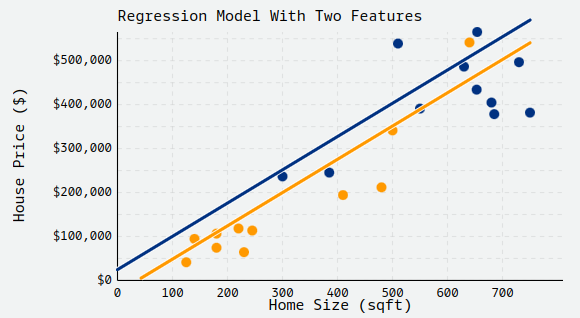
\includegraphics[width=1\linewidth]{../graphs/interpret-3} \end{center}

house price=-27154+757\emph{sqft+51867}pool

\begin{itemize}
\tightlist
\item
  In our example, we model home prices as a function of both the size of
  the house (sqft) and whether or not it has a pool
\end{itemize}
\end{column}

\begin{column}{0.5\textwidth}
\tiny

\begin{itemize}
\item
  intercept: -\$27,154, the predicted average housing price for houses
  with all x\textsubscript{i} = 0. Or the cost of houses with no pools
  and a square-footage of zero.
\item
  coefficient of pool: \$51,867, average expected price difference in
  houses of the same size (in sqft) if they do or do not have a pool. In
  other words, we expect, on average, houses of the same size to cost
  \$51,867 more if they have a pool than if they do not.
\item
  coefficient of sqft: \$757, average expected price difference in
  housing price for houses that have the same value of pool but differ
  in size by one square-foot.
\item
  We assume the same slope for sqft.Hence, two lines. This isn't always
  a valid assumption to make.
\end{itemize}
\end{column}
\end{columns}

\section{Gauss-Markov Theorem}

\end{frame}

\begin{frame}{Gauss-Markov Theorem}
\protect\hypertarget{gauss-markov-theorem}{}

\begin{itemize}
\tightlist
\item
  It is possible to prove that OLS is precise and optimal (BLUE)
\end{itemize}

\begin{block}{Best Linear Unbiased Estimator (BLUE)}

\begin{enumerate}
\tightlist
\item
  The parameters are \emph{linear}
\item
  The parameters are \emph{unbiased}
\item
  The parameters are \emph{efficient}. In other words, they have the
  least variance of all unbiased linear estimators, \emph{best}.
\end{enumerate}

\end{block}

\end{frame}

\begin{frame}{The regression model again}
\protect\hypertarget{the-regression-model-again}{}

\begin{columns}[T]
\begin{column}{0.5\textwidth}
\tiny

\[\begin{aligned}
&Y_1=B_1+B_2 X_{21}+B_3 X_{31}+\cdots+B_k X_{k 1}+u_1 \\
&Y_2=B_1+B_2 X_{22}+B_3 X_{32}+\cdots+B_k X_{k 2}+u_2 \\
&\vdots \\
&Y_n=B_1+B_2 X_{2 n}+B_3 X_{3 n}+\cdots+B_k X_{k n}+u_n
\end{aligned}\]

where:

\begin{itemize}
\tightlist
\item
  \(y\) is an \(N \times 1\) vector of observations of the output
  variable (\(N\) is the sample size);
\item
  X is an \(N \times K\) matrix of inputs (K is the number of inputs for
  each observation);
\item
  B is a \(K \times 1\) vector of regression coefficients;
\item
  u is an \(N \times 1\) vector of errors.\footnote<.->{Taboga, ``Gauss
    Markov Theorem,'' in, \emph{Lectures on probability theory and
    mathematical statistics} (2021).}
\end{itemize}
\end{column}

\begin{column}{0.5\textwidth}
\tiny

Or more succinctly:

\[
\left[\begin{array}{l}
Y_1 \\
Y_2 \\
Y_3 \\
\vdots \\
Y_n
\end{array}\right]=\left(\begin{array}{lll}
1 & X_{21} X_{31} \cdots & X_{k 1} \\
\vdots & \ddots & \vdots \\
1 & X_{2 n} X_{3 n} \cdots & X_{k n}
\end{array}\right)\left[\begin{array}{l}
B_1 \\
B_2 \\
B_3 \\
\vdots \\
B_k
\end{array}\right]+\left[\begin{array}{l}
u_1 \\
u_2 \\
\vdots \\
u_n
\end{array}\right]
\]
\end{column}
\end{columns}

\end{frame}

\begin{frame}{The OLS estimator of \(\beta\) is}
\protect\hypertarget{the-ols-estimator-of-beta-is}{}

\[\hat{\beta} = (X'X)^{-1}X'y\]

\alert{Arriving at this expression}\footnote<.->{Gujarati, ``The
  Classical Linear Regression Model (CLRM),'' in, \emph{Linear
  Regression: A Mathematical Introduction} (2019).}

\begin{block}{OLS is BLUE if it satisfies the assumptions}

\begin{itemize}
\tightlist
\item
  Assumption 1: Linearity. The regression model is linear in the
  parameters; it may or may not be linear in the variables, the Ys and
  Xs.
\end{itemize}

\end{block}

\end{frame}

\begin{frame}{Assumption 2: Regressors are non-stochastic}
\protect\hypertarget{assumption-2-regressors-are-non-stochastic}{}

\begin{itemize}
\tightlist
\item
  The regressors are assumed fixed, or nonstochastic, in the sense that
  their values are fixed in repeated sampling. However, if the
  regressors are stochastic, we assume that each regressor is
  independent of the error term or at least uncorrelated with it.
\item
  X is fixed and exogenous
\item
  X is measured without error
\end{itemize}

\end{frame}

\begin{frame}{Assumption 3: Errors are uncorrelated}
\protect\hypertarget{assumption-3-errors-are-uncorrelated}{}

\begin{columns}[T]
\begin{column}{0.5\textwidth}
\begin{itemize}
\tightlist
\item
  Given the values of the X variables, the expected, or mean, value of
  the error term u is 0.
\end{itemize}

\[E(\epsilon | X) = 0\]
\end{column}

\begin{column}{0.5\textwidth}
\[E\left[\begin{array}{l}
u_1 \\
u_2 \\
u_3 \\
\vdots \\
u_n
\end{array}\right]=\left[\begin{array}{l}
E\left(u_1\right) \\
E\left(u_2\right) \\
E\left(u_3\right) \\
\vdots \\
E\left(u_n\right)
\end{array}\right]=\left[\begin{array}{l}
0 \\
0 \\
0 \\
\vdots \\
0
\end{array}\right]\]
\end{column}
\end{columns}

\end{frame}

\begin{frame}{Assumption 4: Homoscedasticity}
\protect\hypertarget{assumption-4-homoscedasticity}{}

\begin{columns}[T]
\begin{column}{0.5\textwidth}
\begin{itemize}
\tightlist
\item
  The variance of each u, given the values of X, is constant or
  homoscedastic (i.e., of equal variance).
\end{itemize}

\[var(u_i | X) = E(uu')
= \sigma^2I\]
\end{column}

\begin{column}{0.5\textwidth}
\begin{center}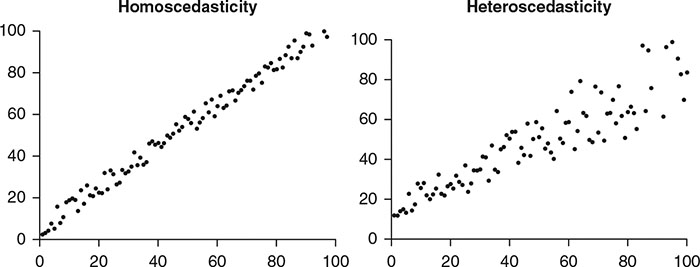
\includegraphics[width=1\linewidth]{../graphs/homosc} \end{center}
\end{column}
\end{columns}

\end{frame}

\begin{frame}{Assumption 5:}
\protect\hypertarget{assumption-5}{}

\begin{itemize}
\tightlist
\item
  There is no correlation between error terms belonging to two different
  observations.
\end{itemize}

\[cov(u_i, u_j | X) = 0\]

Assumption 6: There is no perfect linear relationship among the X
variables. This is the assumption of no multicollinearity.

\end{frame}

\begin{frame}{OLS is linear}
\protect\hypertarget{ols-is-linear}{}

\[\hat{\beta} = (X'X)^{-1}X'y\]

First of all, note that \(\widehat{\beta}\) is linear in \(y\). In fact,
\(\widehat{\beta}\) is the product between the \(K \times N\) matrix
\((X'X)^{-1}X'\) and \(y\), and matrix multiplication is a linear
operation.\footnote<.->{Marcos Taboga, ``Gauss Markov Theorem.''}

\end{frame}

\begin{frame}{OLS is unbiased}
\protect\hypertarget{ols-is-unbiased}{}

\begin{columns}[T]
\begin{column}{0.5\textwidth}
\begin{itemize}
\item
  The true relationship between x and y is: \(y = x\beta + \epsilon\).
\item
  Substituting \textbf{y} into the equation for \(\widehat{\beta}\), we
  get:
\end{itemize}

\[
\begin{aligned}
\widehat{\beta} &= (X'X)^{-1}X'y\\
&= (X'X)^{-1}X'(X\beta + \epsilon)\\
&= (X'X)^{-1}X'x'(X\beta+\epsilon)\\
&= (X'X)^{-1}X'X'X\beta + (X'X)^{-1}X'\epsilon\\
&= I\beta + (X'X)^{-1}X'\epsilon\\
\end{aligned}
\]
\end{column}

\begin{column}{0.5\textwidth}
\[\widehat{\beta} = \beta + (X'X)^{-1}X'\epsilon\]

Take the expected value of the equation:

\[
\begin{aligned}
E(\widehat{\beta}) &= E(\beta + (X'X)^{-1}X'\epsilon)\\
&= \beta + (X'X)^{-1}X'E(\epsilon) \text{Since E(e) = 0}\\
&= \beta\\
\end{aligned}
\]

\begin{itemize}
\tightlist
\item
  Because the expected value of the estimate of \(\beta\) is equal to
  the true value of \(\beta\), the estimator is unbiased
\end{itemize}
\end{column}
\end{columns}

\end{frame}

\begin{frame}{Have the least variance, best}
\protect\hypertarget{have-the-least-variance-best}{}

\begin{columns}[T]
\begin{column}{0.5\textwidth}
\[b^*=\left[A+(X'X)^{-1} X \prime\right] y\]

where A is some nonstochastic k × n matrix, similar to X. Simplifying,
we obtain

\[
\begin{aligned}
&b^*=A y+(X'X)^{-1} X'y \\
&=A y+b
\end{aligned}
\]

where b is the least-squares estimator
\end{column}

\begin{column}{0.5\textwidth}
Now,

\[
\begin{aligned}
&E\left(b^*\right)=\left[A+(X'X)^{-1} X'\right] E(y) \\
&=\left[A+(X'X)^{-1} X \prime\right](X B) \\
&=(A X+I) B
\end{aligned}
\]

Now \(E(b*) = B\) if and only if AX = 0. In other words, for the linear
estimator b* to be unbiased, AX must be 0.
\end{column}
\end{columns}

\end{frame}

\begin{frame}{It has the least variance, best}
\protect\hypertarget{it-has-the-least-variance-best}{}

\begin{columns}[T]
\begin{column}{0.5\textwidth}
\small

Thus,

\[
\begin{aligned}
b^*&=\left[A+(X'X)^{-1} X \prime\right][X B+u], \text{substituting for } (y) \\
&=B+[A+(X'X) X-1 \prime] u \text{, because } A X=0
\end{aligned}
\]

Given that u has zero mean and constant variance (\(=\sigma^2I\)), we
can now find the variance of b* as follows:
\end{column}

\begin{column}{0.5\textwidth}
\small

\[
\begin{aligned}
\operatorname{cov}\left(b^*\right)&=E\left[A+(X \prime X)^{-1} X \prime\right] u u \prime\left[A+(X \prime X)^{-1} X^{\prime}\right] \prime \\
&=\left[A+(X \prime X)^{-1} X \prime\right] E(u u \prime)\left[A+(X \prime X)^{-1} X \prime\right] \prime \\
&=\sigma^2\left[A A \prime+(X \prime X)^{-1}\right] \\
&=\sigma^2(X \prime X)^{-1}+A A \prime \sigma^2 \\
&=\operatorname{var}(b)+A A \prime \sigma^2
\end{aligned}
\]

\begin{itemize}
\tightlist
\item
  shows that the covariance matrix of b* is equal to the covariance
  matrix of b plus a positive semidefinite matrix
\end{itemize}
\end{column}
\end{columns}

\end{frame}

\begin{frame}{Best Linear Unbiased Estimator (BLUE)}
\protect\hypertarget{best-linear-unbiased-estimator-blue-1}{}

\begin{enumerate}
\tightlist
\item
  The parameters are \emph{linear} \[(X'X)^{-1}X'\]
\item
  The parameters are \emph{unbiased} \[E(b) = B\]
\item
  The parameters have the least variance of all unbiased linear
  estimators, \emph{best}.
  \[\widehat{\beta}^{*} = var - cov(\widehat{\beta}) + \sigma^2AA'\]
\end{enumerate}

\end{frame}

\begin{frame}[standout]{}
\protect\hypertarget{section-2}{}

\begin{itemize}
\tightlist
\item
  ALT-TAB to Excel, linear estimator example
\end{itemize}

\end{frame}

\begin{frame}{Conclusion}
\protect\hypertarget{conclusion}{}

\begin{itemize}
\tightlist
\item
  We saw a review of linear regression
\item
  How multivariate regression works
\item
  And how OLS is the best of the linear estimators
\end{itemize}

\end{frame}

\begin{frame}{Acknowledgements}
\protect\hypertarget{acknowledgements}{}

\begin{columns}[T]
\begin{column}{0.5\textwidth}
\begin{block}{Team}

\begin{itemize}
\tightlist
\item
  Joshua Pritkin.
\item
  Rob Kirkpatrick.
\end{itemize}

\vspace{3mm}

\begin{itemize}
\item
  Michael C Neale.
\item
  NIH grant no R01 DA049867 and 5T32MH-020030
\end{itemize}

\end{block}
\end{column}

\begin{column}{0.5\textwidth}
\begin{block}{Contact}

\begin{center}
\includegraphics[width=0.8\linewidth]{../graphs/qr-twitter-1} \end{center}

\end{block}
\end{column}
\end{columns}

\appendix

\end{frame}

\begin{frame}[standout]{}
\protect\hypertarget{section-3}{}

\begin{itemize}
\tightlist
\item
  Thank you
\end{itemize}

\end{frame}

\begin{frame}{Interpretation 4}
\protect\hypertarget{interpretation-4}{}

\begin{center}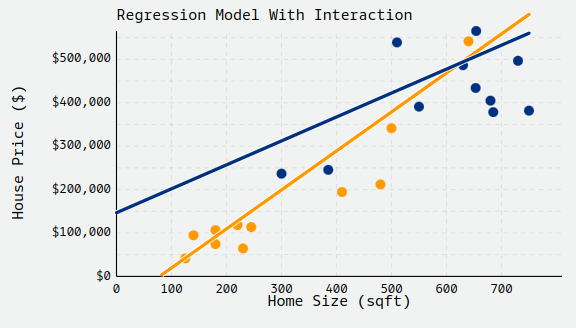
\includegraphics[width=1\linewidth]{../graphs/interpret-4} \end{center}

\end{frame}

\begin{frame}{What it means to be best}
\protect\hypertarget{what-it-means-to-be-best}{}

Now that we have shown that the OLS estimator is linear and unbiased, we
need to prove that it is also the best linear unbiased estimator.

\begin{block}{What exactly do we mean by best?}

When \(\widehat{\beta}\) is a scalar (i.e., there is only one
regressor), we consider \(\widehat{\beta}\) to be the best among those
we are considering (i.e., among all the linear unbiased estimators) if
and only if it has the smallest possible variance, that is, if its
deviations from the true value \(\beta\) tend to be the smallest on
average. Thus, \(\widehat{\beta}\) is the best linear unbiased estimator
(BLUE) if and only if

\[Var[\widehat{\beta}|X] \leq Var[\widetilde{\beta}|X]\]

for any other linear unbiased estimator \(\widetilde{\beta}\).

\end{block}

\end{frame}

\begin{frame}{What it means to be best}
\protect\hypertarget{what-it-means-to-be-best-1}{}

Since we often deal with more than one regressor, we have to extend this
definition to a multivariate context. We do this by requiring that

\[Var[\alpha\widehat{\beta}|X] \leq Var[\alpha\widetilde{\beta}|X]\]

for any \(1 \times K\) constant vector \(\alpha\), any other linear
unbiased estimator \(\widetilde{\beta}\).

In other words, OLS is BLUE if and only if any linear combination of the
regression coefficients is estimated more precisely by OLS than by any
other linear unbiased estimator.

\end{frame}

\begin{frame}{What it means to be best}
\protect\hypertarget{what-it-means-to-be-best-2}{}

Condition (1, previous) is satisfied if and only if

\[Var[\widetilde{\beta}|X] - Var[\widehat{\beta}|X]\]

is a positive semi-definite matrix.

In the next two sections we will derive \(Var[\widehat{\beta}|X]\) (the
covariance matrix of the OLS estimator), and then we will prove that (2,
above) is positive-semidefinite, so that OLS is BLUE.

\end{frame}

\begin{frame}{The covariance matrix of the OLS estimator}
\protect\hypertarget{the-covariance-matrix-of-the-ols-estimator}{}

The conditional covariance matrix of the OLS estimator is

\[Var[\widehat{\beta}|X] = \sigma^2(X'X)^{-1}\]

\end{frame}

\begin{frame}{OLS is BLUE}
\protect\hypertarget{ols-is-blue}{}

Since we are considering the set of linear estimators, we can write any
estimator in this set as

\[\widetilde{\beta} = Cy\]

where \(C\) is a \(K \times N\) matrix.

Furthermore, if we define

\[D = C - (X'X)^{-1}X'\]

\end{frame}

\begin{frame}{OLS is BLUE}
\protect\hypertarget{ols-is-blue-1}{}

then we can write

\[\begin{aligned}\widetilde{\beta} &= Cy\\
                    &= Dy + (X'X)^{-1}X'y\\
                    &= Dy + \widehat{\beta}
                    \end{aligned}\]

It is possible to prove that \(DX=0\) if \(\widetilde{\beta }\) is
unbiased.

\end{frame}

\begin{frame}{OLS is BLUE}
\protect\hypertarget{ols-is-blue-2}{}

By using this result, we can also prove that

\[Var[\widehat{\beta}|X] = Var[\widetilde{\beta}|X] + \sigma^2DD'\]

As a consequence,

\[Var[\widehat{\beta}|X] - Var[\widetilde{\beta}|X] + \sigma^2DD'\]

is positive semi-definite because {[}eq28{]} is positive semi-definite.
This is true for any unbiased linear estimator \(widetilde{\beta }\).
Therefore, the OLS estimator is BLUE.

\end{frame}

\begin{frame}{It has the least variance, best}
\protect\hypertarget{it-has-the-least-variance-best-1}{}

\begin{columns}[T]
\begin{column}{0.5\textwidth}
\small

Thus,

\[
\begin{aligned}
b^*&=\left[A+(X'X)^{-1} X \prime\right][X B+u], \text{substituting for } (y) \\
&=B+[A+(X'X) X-1 \prime] u \text{, because } A X=0
\end{aligned}
\]

Given that u has zero mean and constant variance (\(=\sigma^2I\)), we
can now find the variance of b* as follows:
\end{column}

\begin{column}{0.5\textwidth}
\small

\[
\begin{aligned}
\operatorname{cov}\left(b^*\right)&=E\left[A+(X \prime X)^{-1} X \prime\right] u u \prime\left[A+(X \prime X)^{-1} X^{\prime}\right] \prime \\
&=\left[A+(X \prime X)^{-1} X \prime\right] E(u u \prime)\left[A+(X \prime X)^{-1} X \prime\right] \prime \\
&=\sigma^2\left[A A \prime+(X \prime X)^{-1}\right] \\
&=\sigma^2(X \prime X)^{-1}+A A \prime \sigma^2 \\
&=\operatorname{var}(b)+A A \prime \sigma^2
\end{aligned}
\]

\begin{itemize}
\tightlist
\item
  shows that the covariance matrix of b* is equal to the covariance
  matrix of b plus a positive semidefinite matrix
\end{itemize}
\end{column}
\end{columns}

\end{frame}

\begin{frame}{OLS is unbiased}
\protect\hypertarget{ols-is-unbiased-1}{}

\begin{columns}[T]
\begin{column}{0.5\textwidth}
\[
\begin{aligned}
b &=(X'X)^{-1} X'y \\
&=(X'X)^{-1} X'[X B+u], \text { substituting for } y \\
&=(X'X)^{-1} X'X B+(X'X)^{-1} X'u \\
&=B+(X'X)^{-1} X'u
\end{aligned}
\]

Now,

\[
\begin{aligned}
E(b)&=B+(X'X)^{-1} X^{\prime} E(u) \\
&=B
\end{aligned}
\]
\end{column}

\begin{column}{0.5\textwidth}
In words, the expected value of b is equal to B, thus proving that b is
unbiased. (Recall the definition of unbiased estimator.) Note that
\(E(u|X) = 0\) by assumption.
\end{column}
\end{columns}

\end{frame}

\end{document}
